\documentclass[11pt]{article}   	% use "amsart" instead of "article" for AMSLaTeX format
%\usepackage{geometry}                		% See geometry.pdf to learn the layout options. There are lots.
%\geometry{letterpaper}                   		% ... or a4paper or a5paper or ... 
%\geometry{landscape}                		% Activate for for rotated page geometry
\usepackage[parfill]{parskip}    		% Activate to begin paragraphs with an empty line rather than an indent

\usepackage{graphicx}				% Use pdf, png, jpg, or eps� with pdflatex; use eps in DVI mode
								% TeX will automatically convert eps --> pdf in pdflatex		
\usepackage{amssymb}
\usepackage[top=1.1in, bottom=1.1in, right=1.0in, left=1.0in]{geometry}
\usepackage{fancyhdr}
\usepackage{titling}
\usepackage{authblk}
%\usepackage{natbib}
\usepackage{cite}
\usepackage[labelformat = empty,position=top]{subcaption}
\usepackage[export]{adjustbox}
\usepackage{float}
\usepackage[hidelinks]{hyperref}
\hypersetup{
    linktoc=all
}
\usepackage[aboveskip=1pt,labelfont=bf,labelsep=period,singlelinecheck=off,size=small]{caption}

%\usepackage[round]{natbib}
%\bibliographystyle{plainnat}

\bibliographystyle{ieeetr}

\usepackage{color}
\newcommand*{\edit}[1]{{\bfseries\textcolor{red}{#1}}}

\newcommand{\Expo}{\textrm{Expo}}

\setlength{\droptitle}{-1in}
\title{Theory Paper: Supplementary Information}
\author{Grant Kinsler, Kerry Geiler-Samerotte, Dmitri Petrov}
\date{}

\begin{document}
\maketitle

%\tableofcontents
%\thispagestyle{empty}

%\setcounter{page}{1}
\section{Mathematical and Computational Details}
\subsection{Guassian fitness function uniquely satisfies desired properties}

One important consideration of our use of fitness to identify phenotypes is the mapping between the two, in particular the fitness function. There are many choices for such a function, each with various properties that make them appropriate and preferred in certain contexts. \edit{Some sentences here about use in various cases - linear, gaussian, others?}. 

For our particular case, identifying fitness-relevant phenotypes, one particular property that seems desirable is that a trait only contributes to relative fitness if the ancestor and mutant differ in their trait value for that particular trait, since this means we will only identify differing traits when using fitness do identify them. As we show below, if fitness is a function of Euclidean distance in phenotype space, then the only class of functions that satisfies this property is that of an exponential function of squared distance, such as the Gaussian function.

% In our case, one property that may desirable is that for a phenotype to have an impact on relative fitness between the ancestor and a mutant, the ancestor and mutant must differ in their values of that phenotype. This allows us to restrict our analysis to only phenotypes that differ. Mathematically, this property means that phenotypes are independent in their contribution to fitness
%
%This is a nice mathematical property and it seems like a desirable quality for any fitness function we might want to use. Unfortunately (as I will show), this class of functions is the only class of function that has this property, so we should think more deeply about if we think this is a necessary property for a fitness function (and perhaps what assumptions about the space we're implicitly making by using this function).

Consider a phenotype space with 2 dimensions. Let the ancestor and mutant both lie solely in the first dimension with distance $ x_A $ and $ x_M $ from the optimum's projection in this dimension. The optimum also has a non-zero value $ y $ in the second dimension (without loss of generality, we can set 0 to be the value shared by the ancestor and mutant in this dimension) (see Figure 1). 

\begin{figure}[ht]
\begin{center}
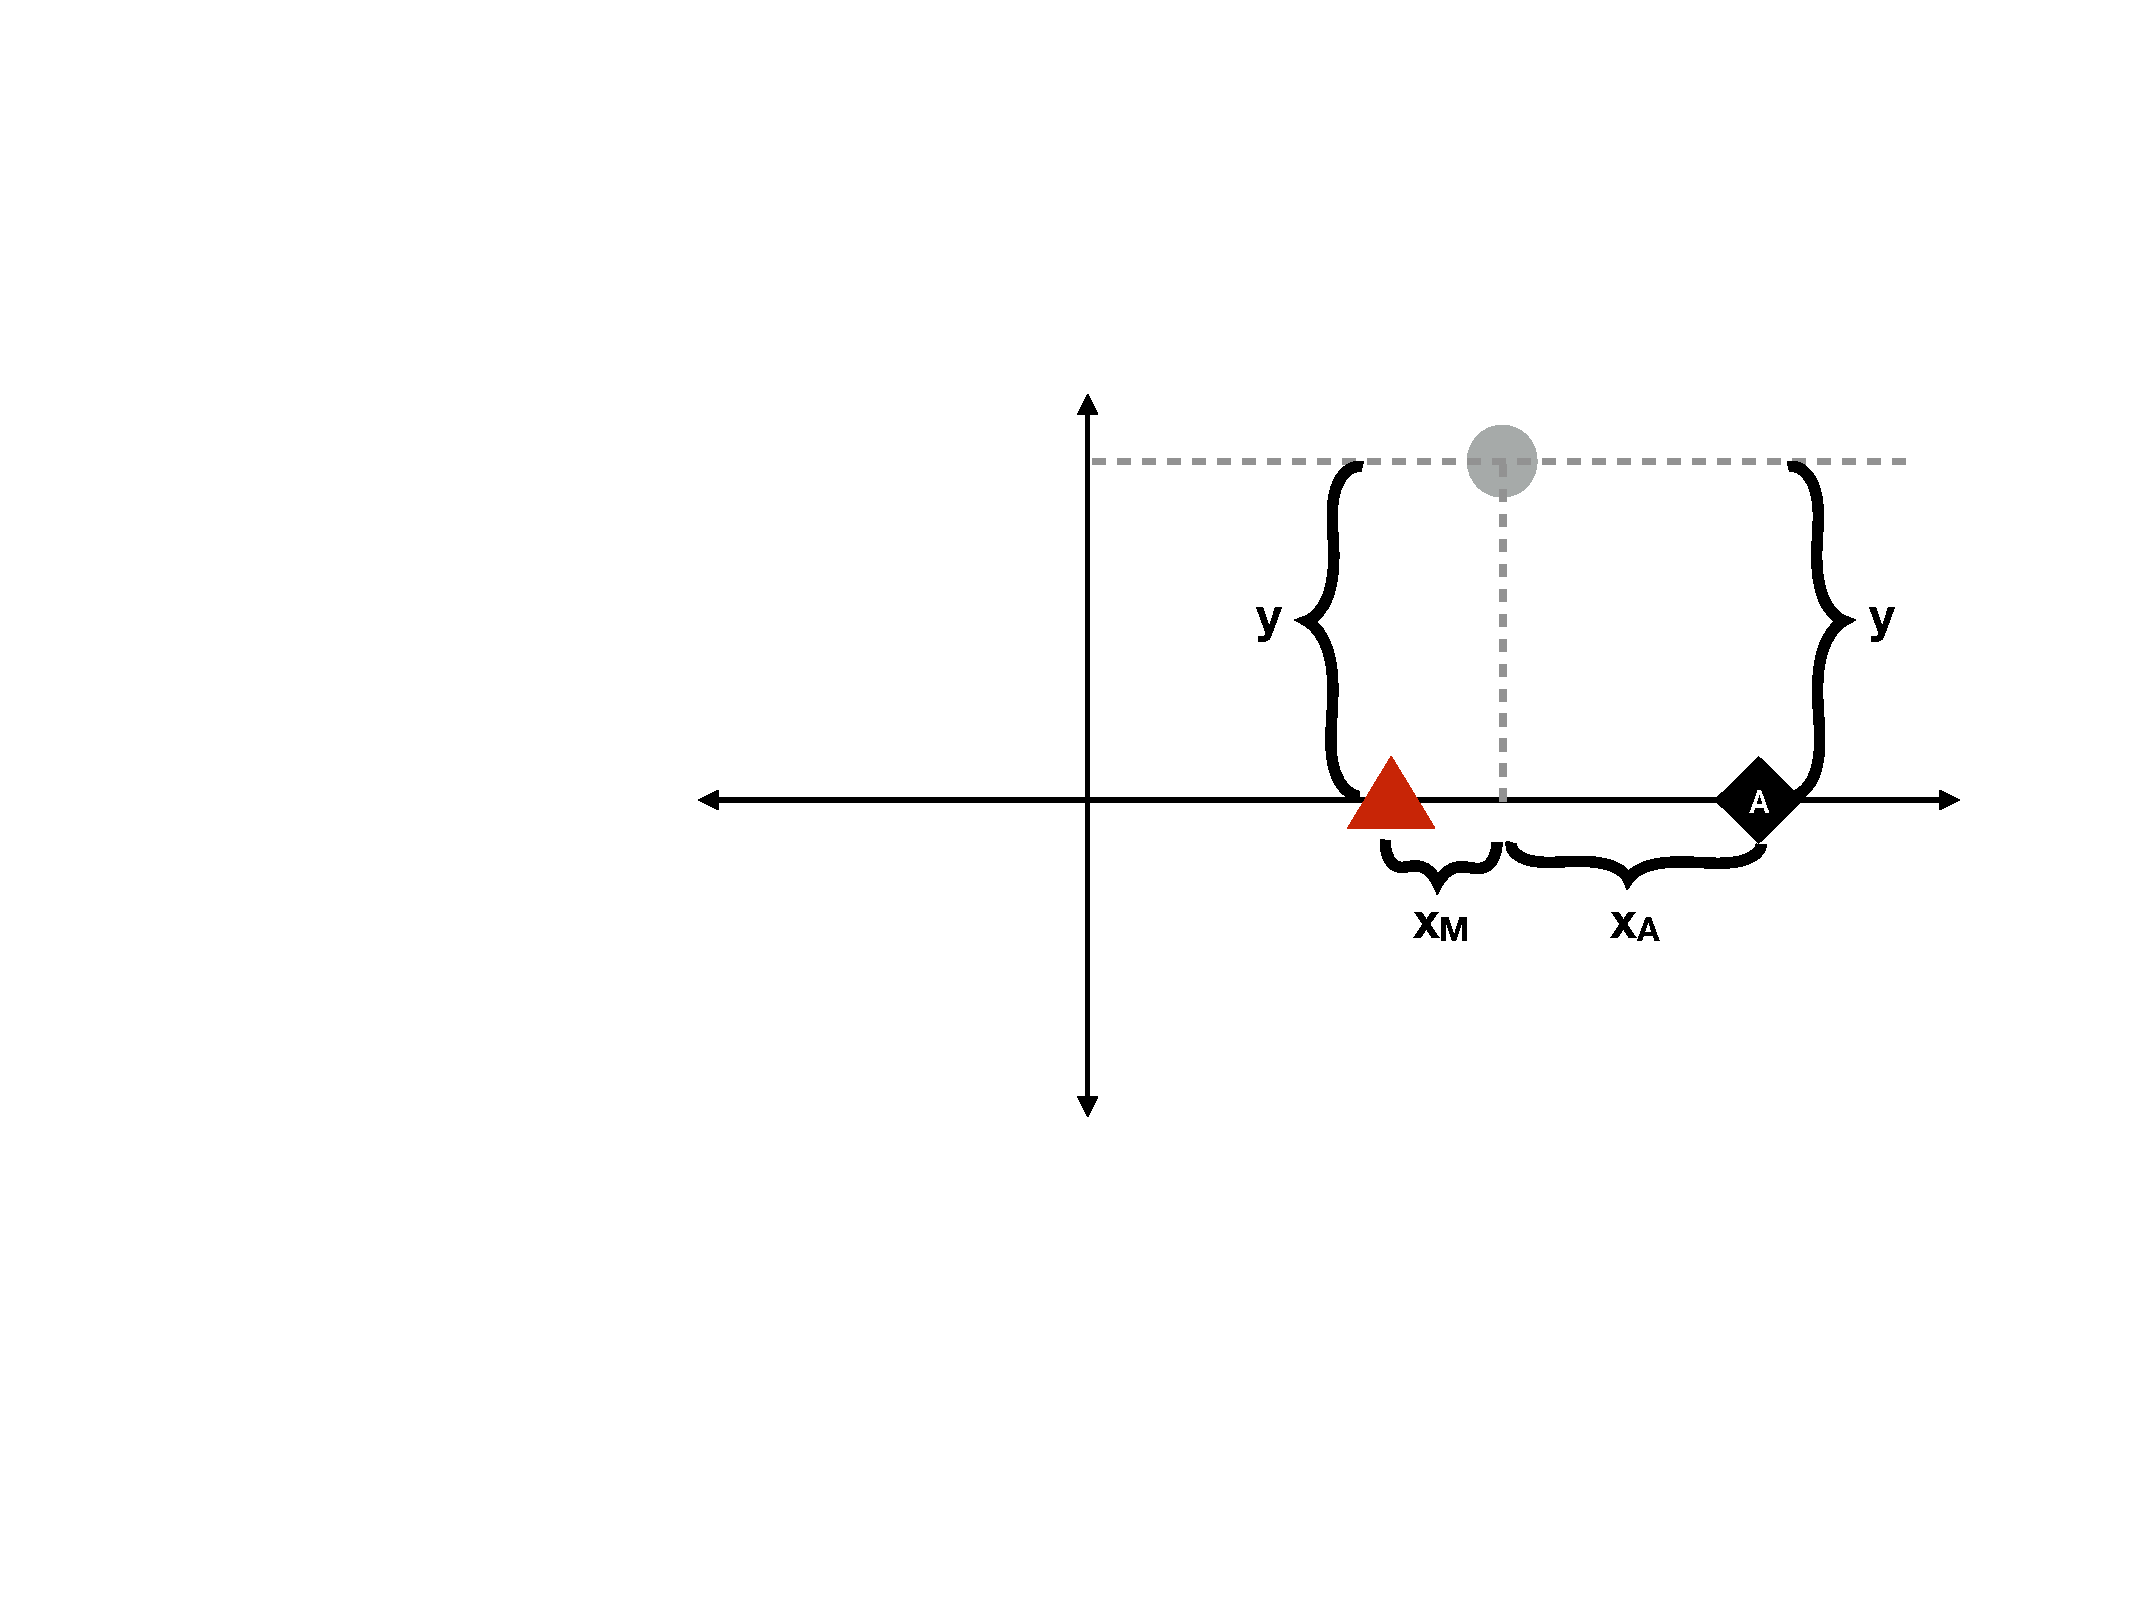
\includegraphics[width=4in]{figures/distance_figure.pdf}
\end{center}
\caption{{\bf Graphical illustration of distance properties.} The ancestor (black diamond) and mutant (red triangle) differ in their trait value in the first dimension but not the second. The condition's optimum (gray circle) differs from both the ancestor and mutant in both dimensions.}
\end{figure}



Let the fitness function be some function of Euclidean distance in phenotype space. We can calculate the Euclidean distance of the mutant and ancestor from the optimum:
\[ d_{M} = \sqrt{x_{M}^2 + y^2}  \qquad d_{A} = \sqrt{x_{A}^2 + y^2} \]

In general, relative fitness is given by:
\[ s = \frac{w_{M} - w_{A}}{w_{A}} = \frac{w_{M}}{w_{A}} -1 \]

where  $ w_M = f( d_{M} ) $ is some function of the distance from the optimum (with same function for the ancestor). Essentially, we want to find functions $ f $ such that there is no $ y $ in the simplified expression for $ s $:
\[ s = \frac{w_{M}}{w_{A}} -1 =  \frac{f\left( \sqrt{x_{M}^2 + y^2}  \right)}{f\left( \sqrt{x_{A}^2 + y^2}  \right)} -1 \]
One thing to notice is that we cannot keep \( y \) in the denominator. If \( y \) is kept in the denominator, it will always participate in scaling fitness (and thus have an influence on relative fitness), so we need a function that removes the distance from the ancestor such that \( f(d_M)/f(d_A) = f(d_M-d_A) \). There is only one such class of real-valued, positive functions that has this property, which is the exponential \edit{[this is a classic Real Analysis course proof - what's a good citation?]}, meaning our function must have the form \( f(d_M) = \exp(g(d_M)) \). This gives us:
\( s = \exp\left[  g\left(  \sqrt{x_{M}^2 + y^2}  \right) -  g\left(  \sqrt{x_{A}^2 + y^2} \right)   \right] \).
We can now see that the \( g \) function must be quadratic to remove the square root allow for \( y \) itself to cancel out. This means that in order to satisfy the property of not depending on the extra dimension where the mutants do not differ from the ancestor, we need an absolute fitness function that is the exponential of the squared distance from the optimum - the Gaussian function satisfies this property.

\subsection{Derivation of Score Metric}

To derive the score (eq. 1) used in the main text, we assume that fitness for mutant $ j $ at position $ \vec{x}_j $ in condition $ k $ is given by:
\begin{equation}
F_{jk}= \frac{h_k}{\sqrt{2\pi\sigma_k^2}}\exp\left( -\frac{\sum_{i=1}^D \left( x_{ij} - o_{ik} \right)^2}{2\sigma_k^2} \right)
\end{equation}
where fitness in condition $ k $ is represented by a Gaussian function centered at $ \vec{o}_k $, with height $ h_k $ and variance $ \sigma_k^2 $. Using this absolute fitness function, relative fitness from an ancestor at the location $ \vec{a} $ is given by:
\begin{equation}
 f_{jk} = \frac{F_{jk}}{F_{Ak}} - 1 = \frac{\exp\left( -\frac{\sum_{i=1}^D \left( x_{ij} - o_{ik} \right)^2}{2\sigma_k^2} \right)}{\exp\left( -\frac{\sum_{i=1}^D \left( a_{i} - o_{ik} \right)^2}{2\sigma_k^2} \right)} - 1 = \exp\left( \frac{\sum_{i=1}^D \left( a_{i} - o_{ik} \right)^2 - \sum_{i=1}^D \left( x_{ij} - o_{ik} \right)^2}{2\sigma_k^2} \right) - 1 
 \end{equation}
Note that the height of the Gaussian $ h_k $ drops out of the equation for relative fitness. To find values of the parameters (including location of the mutants, optima, and ancestor) that best fit our observed data (the measured relative fitnesses), we need to derive a score that minimizes the difference between the predicted relative fitness given by the model and the observed relative fitness. Since our estimation technique relies on repeatedly evaluating a function of the locations of the mutants, optima, and ancestor, it is computationally costly to have an exponential function in this evaluation. Accordingly, we use a log-transform of this equation to derive our score metric:
\begin{equation}
S\left(x,o,a|f,\epsilon \right) = \sum_{j=1}^M \sum_{k=1}^C \epsilon_{jk} \left[ \left( \sum_{i=1}^D \left(a_{i} - o_{ik}\right)^2 - \sum_{i=1}^D \left(x_{ij} - o_{ik}\right)^2 \right) - 2 \sigma_{k}^2 \log\left[ 1+f_{jk} \right] \right]^2
\end{equation}
where the $ \epsilon_{jk}$ is weighting for measurement error according to relative inverse variance weighting, such that:
\[ \epsilon_{jk} =  \frac{\frac{1}{s_{jk}^2}}{\sum_{j,k} \frac{1}{s_{jk}^2}}  \]
where $ s_{jk}^2 $ is the sampling variance for the given measurement [CITE venkataram supplement?]. 

\subsection{Constraining symmetry}

There are a number of symmetric solutions that can fit this solution. We constrain symmetry and reduce the number of parameters that we fit by the ancestor to the location $ \left( a, 0, \dots , 0 \right) $ and optima such that the first optimum is at the origin, and the $ d $th optimum is constrained to the $ d $-dimensional Euclidean subspace (up until the $ D $th optimum, whereafter each optimum has all $ D $ values). After imposing these constraints, and fixing the variance of the Gaussian to $ \sigma_k^2 = 1.0 $, we can calculate the total number of variables in our optimization problem to understand when the problem becomes underdetermined. We need the number of variables to be less than the number of data points (which is given by $ M C$). Thus we are overdetermined (and okay solving the problem if):
\[ M(D) + (C-D)D + \frac{D(D+1)}{2}  < M C \]
When there are many more mutants than conditions, then the terms with $ M $ dominate, and the problem is feasible when the number of dimensions is less than the number of conditions included.

%where $ \vec{x}_j $ is a vector representing the location of genotype $ j $, $ o_k $ represents the location of the optimum of environment $ k $, $ \sigma_k^2 $ is the variance of the Gaussian fitness function, and $ D $ is the number of phenotypic dimensions being evaluated. Since we measure fitness relative to the ancestor, we can translate to the relative fitness of genotype $ j $ in environment $ k $:
%
%\begin{equation} 
%%f_{jk} = \frac{W_{k}\left( \vec{x}_j \right)}{W_{k}\left( A \right)} -1 = \frac{\exp\left( -\frac{\sum_{i=1}^D \left( x_{ij} - o_{ik} \right)^2}{2\sigma^2} \right)}{\exp\left( -\frac{\sum_{i=1}^D \left( A_i- o_{ik} \right)^2}{2\sigma^2} \right)} -1 = \exp\left(\frac{\sum_{i=1}^D \left( A_i- o_{ik} \right)^2 - \sum_{i=1}^D \left( x_{ij} - o_{ik} \right)^2}{2\sigma^2}  \right) -1 
%f_{jk} = \frac{F_{k}\left( \vec{x}_j \right)}{F_{k}\left( A \right)} -1 = \exp\left(\frac{\sum_{i=1}^D \left( a_i- o_{ik} \right)^2 - \sum_{i=1}^D \left( x_{ij} - o_{ik} \right)^2}{2\sigma_k^2}  \right) -1 
% \end{equation}
%
%We want to minimize the difference between this fitness value for the model and the measured fitness value. For computational feasibility, we take the log transform of this difference, and perform least squares optimization summing over all mutants and conditions. Thus, we are interested in finding the global minimum of the function:
%
%\begin{equation}
%S\left(x,o,A|f,\epsilon \right) = \sum_{j=1}^M \sum_{k=1}^C \epsilon_{jk} \left[ \left( \sum_{i=1}^D \left(x_{ij} - o_{ik}\right)^2 - \left(  (A-o_{1k})^2 + \sum_{i=2}^D o_{ik}^2   \right) \right) - 2 \log\left[ 1+f_{jk} \right] \right]^2
%\end{equation}



%There are a number of symmetric solutions that can fit this solution. We constrain symmetry and reduce the number of parameters that we fit by the ancestor to the location $ \left( A, 0, \dots , 0 \right) $ and optima such that the first optimum is at the origin, and the $ d $th optimum is constrained to the $ d $-dimensional Euclidean subspace (up until the $ D $th optimum, whereafter each optimum has all $ D $ values). After imposing these constraints, and fixing the variance of the Gaussian to $ \sigma_k^2 = 1.0 $, we can calculate the total number of variables in our optimization problem to understand when the problem becomes underdetermined. We need the number of variables to be less than the number of data points (which is given by $ M C$). Thus we are overdetermined (and okay solving the problem if):
%\[ M(D) + (C-D)D + \frac{D(D+1)}{2}  < M C \]
%When there are many more mutants than conditions, then the terms with $ M $ dominate, and you need approximately one more condition than the number of dimensions you'd like to estimate.

\subsection{Optimization Implementation}

To find the best possible solution to this nonlinear optimization problem, we use a global minimization technique implemented in Python. In particular, we use \texttt{scipy.optimize.basinhopping}, which combines gradient descent with random displacement to find various local minima. Local minima are accepted similarly to Metropolis-Hastings and Simulated Annealing approaches, and the process continues to iterate until the number of steps has been completed. We run numerous simulations from random starting locations and compare the found solutions to ensure consistency in our optima. However, because this is a global optimization technique, there is no guarantee that the solution we find is the best possible one. Thus, our solutions should be seen as the best local optimum found. Because of this, substantial simulations are needed to confirm the robustness of this model and its implementation.

\subsection{Simulation Implementation}

To generate simulation data, we uniformly draw points from within the $ n$-dimensional ball according to the Marsaglia Algorithm \cite{Marsaglia1972}





\end{document}  